\documentclass{article}
\usepackage{amsmath}
\usepackage{MnSymbol}
\usepackage{wasysym}
\usepackage[toc,page]{appendix}
\usepackage{hyperref}
\usepackage{graphicx}
\usepackage{float}
\usepackage[numbered,framed]{matlab-prettifier}
\usepackage[export]{adjustbox}
\begin{document}
	\begin{center}
		\LARGE \bfseries{Answers to Problem Set 4}\\
		Group name: Ferienspass\vspace{.5cm}\\
		\normalsize \normalfont
		Sebastian K\"uhnl: 5642348\\
		Alexander D\"uck (as: reebyte): 5504077\\
		Patrick Blank (as: paddyblank): 6729110\\
		Christian Wierschem: 6729288
	\end{center}
	\normalsize	
	\section{Question 1}
	Chebyshev approximation using equidistant nodes and Chebyshev nodes. However, there is a difference between lecture slides 7 and the notes from te lecture, as you will see in the code: 
	\lstinputlisting[style=Matlab-editor]{cheb.m}
	Linear and cubic splines, also using the Miranda-Fackler toolbox:
	\lstinputlisting[style=Matlab-editor]{spl.m}
	The function, which was given in the task, defined for potential vector input:
	\lstinputlisting[style=Matlab-editor]{simplef.m}
	Main code for PS4P1:
	\lstinputlisting[style=Matlab-editor]{PS4P1.m}
	Plots are ordered in chronological order! (For comparison, the residuals to actual function are plotted.)\\
	\begin{figure}[h]
	  \begin{minipage}{0.56\textwidth}
	  	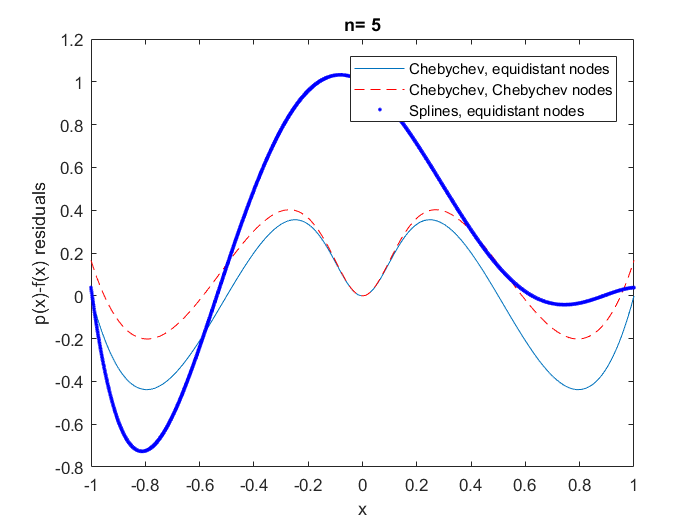
\includegraphics[width = \textwidth, keepaspectratio]{n5res.png}
	  \end{minipage}
	  \begin{minipage}{0.56\textwidth}
	    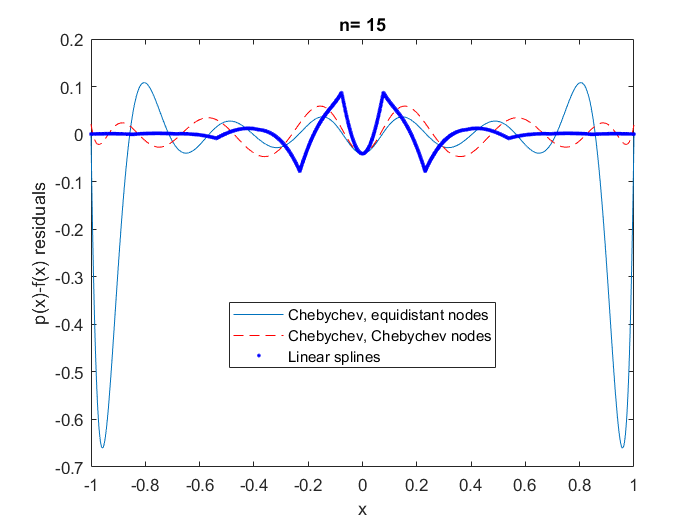
\includegraphics[width = \textwidth, keepaspectratio]{n15res.png}
      \end{minipage}
   	  \begin{minipage}{0.56\textwidth}
   	  	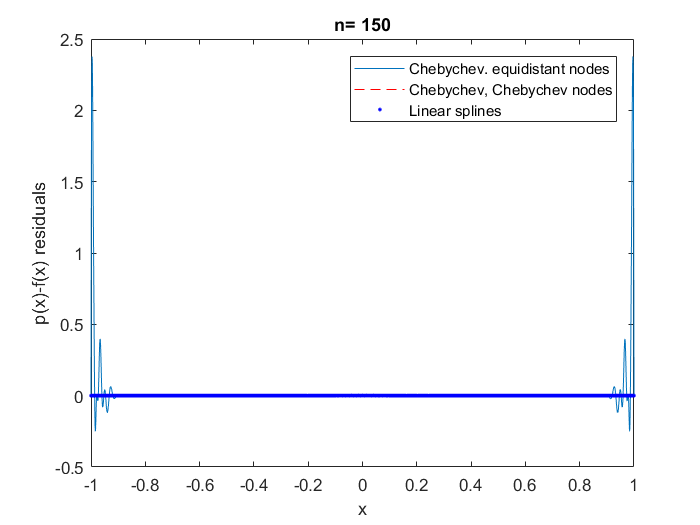
\includegraphics[width = \textwidth, keepaspectratio]{n150res.png}
   	  \end{minipage}   	   
    \end{figure}\\
   For n=5, equidistant nodes and Chebyshev nodes as well as linear splines are very similar. For n=15, linear splines become more edgy. It performs well at the edges and average else. Both Chebyshev approximations are very similar in [-0.75;0.75], while equidistant nodes fall off at the edges (as expected). For n=150 this effect is even stronger, but it moves closer to the corner. The others are not comparable due to the residual scale. The effect does not occur when using Chebyshev nodes because there are more nodes at the corner to prevent these large fluctuations.\\
	\begin{figure}[h]
	\begin{minipage}{0.56\textwidth}
	  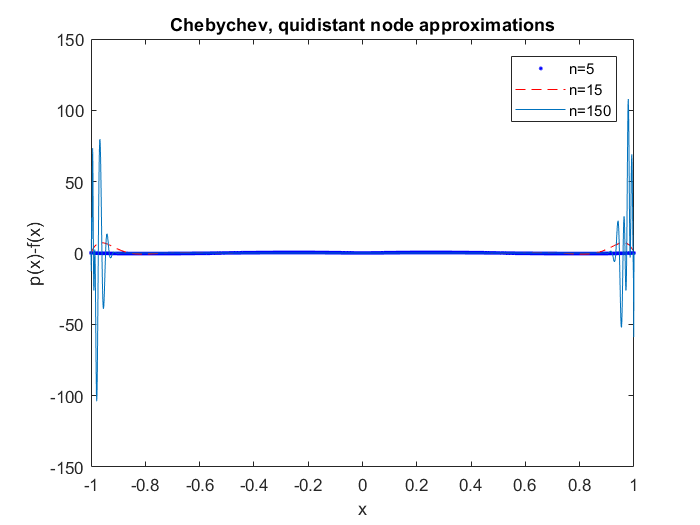
\includegraphics[width = \textwidth, keepaspectratio]{chebequi.png}
    \end{minipage}
    \begin{minipage}{0.56\textwidth}
	  \includegraphics[width = \textwidth, keepaspectratio]{chebcheb.png}
    \end{minipage}
    \begin{minipage}{0.56\textwidth}
	  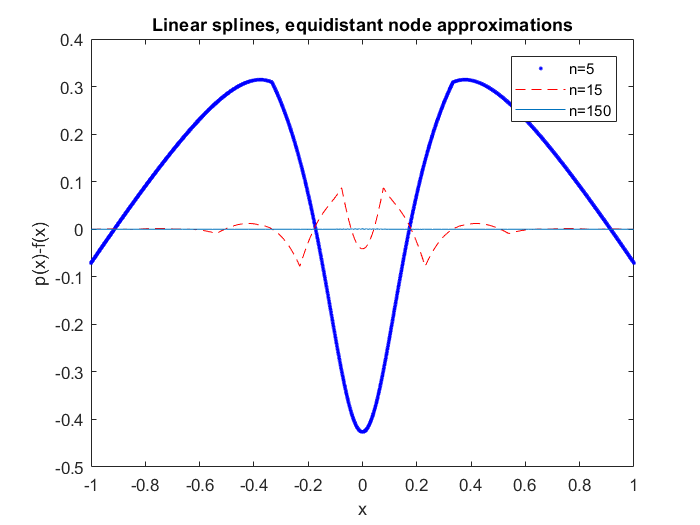
\includegraphics[width = \textwidth, keepaspectratio]{splequi.png}
    \end{minipage}   	   
    \end{figure}\\
    In this figure again the effect of equidistant nodes when using Chebyshev can be seen as large fluctuations at the corner. Besides this, as the number of nodes increases, the approximation gets closer to the real function.\\
    \newpage
	\begin{figure}[h]
	\begin{minipage}{0.56\textwidth}
	  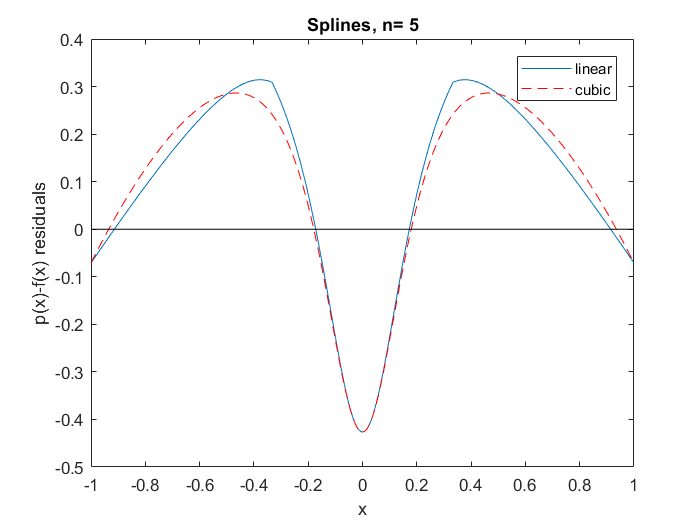
\includegraphics[width = \textwidth, keepaspectratio]{n5lincub.png}
    \end{minipage}
    \begin{minipage}{0.56\textwidth}
	  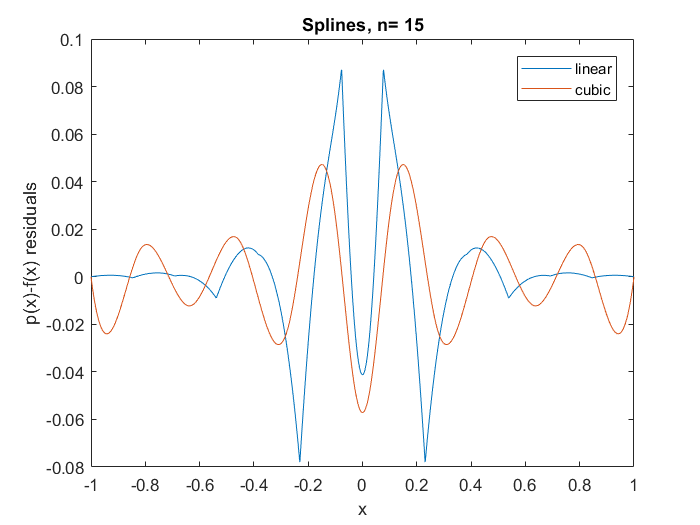
\includegraphics[width = \textwidth, keepaspectratio]{n15lincub.png}
    \end{minipage}
    \begin{minipage}{0.56\textwidth}
	  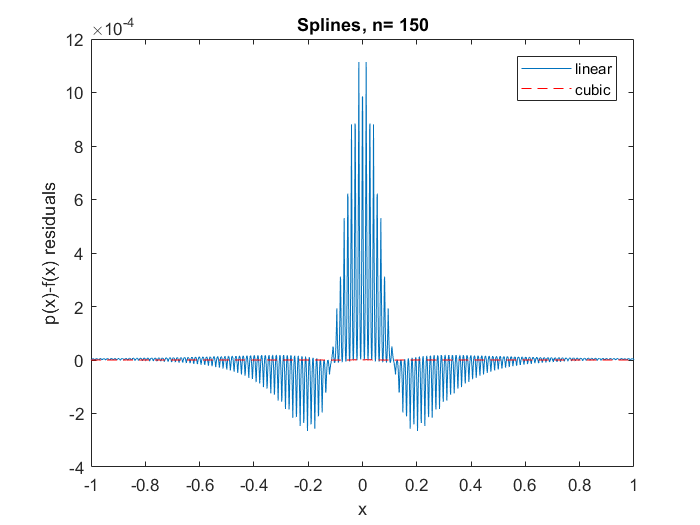
\includegraphics[width = \textwidth, keepaspectratio]{n150lincub.png}
    \end{minipage}   	   
    \end{figure}
    Linear and cubic splines are very similar when n=5. For n=15 one can observe that cubic splines are smoother than linear splines and perform better in the center (around 0), whereas linear splines perform better at the corner (it becomes smooth and then becomes nearly a straight line). For n=150, at first sight, linear splines perform badly, but it is only relative to cubic splines (look at the scale). As n increases, the approximation gets better when using splines.\\
    \newpage
	\begin{figure}[h]
	\begin{minipage}{0.56\textwidth}
	  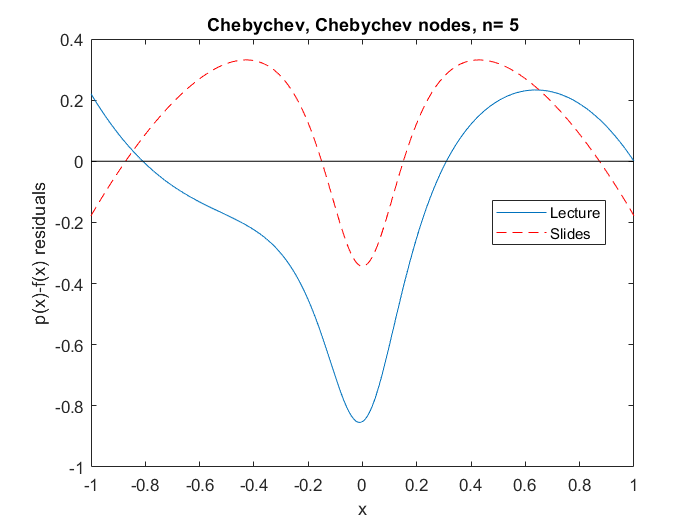
\includegraphics[width = \textwidth, keepaspectratio]{n5lecsli.png}
    \end{minipage}
    \begin{minipage}{0.56\textwidth}
	  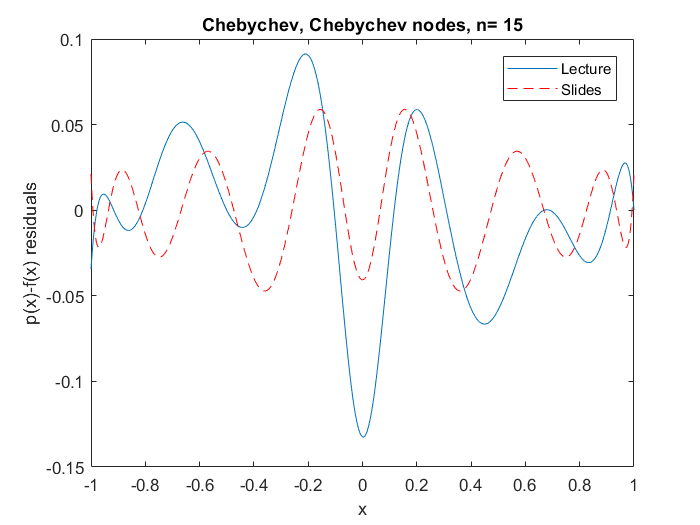
\includegraphics[width = \textwidth, keepaspectratio]{n15lecsli.png}
    \end{minipage}
    \begin{minipage}{0.56\textwidth}
	  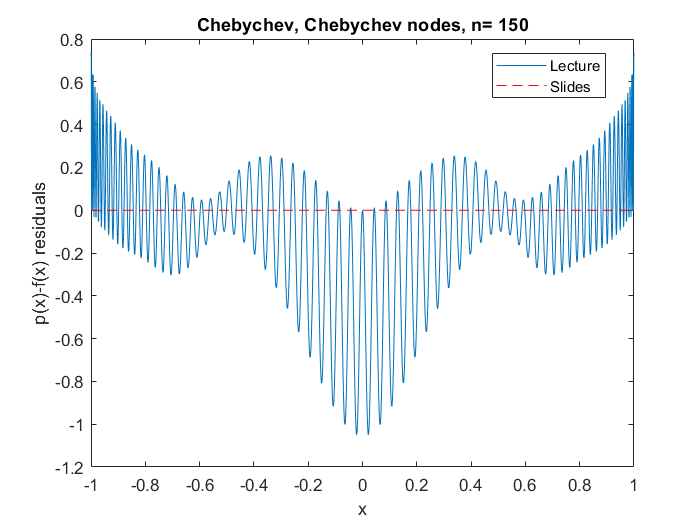
\includegraphics[width = \textwidth, keepaspectratio]{n150lecsli.png}
    \end{minipage}   	   
    \end{figure}
    The slides formula seems to be the right one. The function is symmetric and so is the approximation. The lecture formula leads to very odd (i.e. asymmetric) approximations.\\\\
    In general, it seems to be very odd that the residuals at 0 are not 0, because there should be a node and thus the residual should be zero. Maybe it is due to the toolbox calculations. Other possibilities have been thought of and precluded.
\newpage
	\section{Question 2}

\end{document}